\chapter{Experiment Description and PCC method}
 
 General-purpose detectors used in high-energy colliders have cylindrical detection layers that are arranged around the beam axis. The Compact Muon Solenoid (CMS), which is one of the largest international scientific collaborations in history and is part of the LHC at CERN, is an example of such a detector. The CMS detector is designed to carry out a wide range of experiments that include studying the Standard Model. This chapter provides a description of the various components of the CMS detector, including the several systems to measure the luminosity with a particular focus on the silicon pixel tracker, which is described in greater detail due to its relevance to this work.
 
\section{The Compact Muon Solenoid}

The CMS experiment is a general purpose detector and is part of the LHC's four detectors. This detector is built around a massive cylindrical solenoid magnet, which is made of superconducting cable that produces a powerful magnetic field of 4 tesla. This magnetic field is utilized to distinguish the energy deposits of charged and neutral particles in jets within the calorimeter. The magnet's field is confined by a steel "yoke," which comprises most of the detector's mass, totaling 14,000 tonnes. The CMS detector itself has dimensions of 21.6 meters in length and 14.6 meters in diameter \cite{CMS_Exp_2008}.\\

The CMS detector comprises various detection layers that include separate parts of the detector, these layers are the fine-grained silicon tracker, which provides efficient and precise reconstruction of charged-particle trajectory. The highly-segmented electromagnetic calorimeter (ECAL) wish principal purpose is the detection of  electromagnetic energy and the identification of electrons and photons. The hadronic calorimeter (HCAL) wish principal purpose is the detection of hadrons in jets  \cite{CMS_Exp_2008}. Additionally, there is an excellent muon tracking system. A schematic representation of the CMS detector is shown in Fig. \ref{detector_CMS}.

\begin{center}
  \begin{figure}[ht]
    \centering
    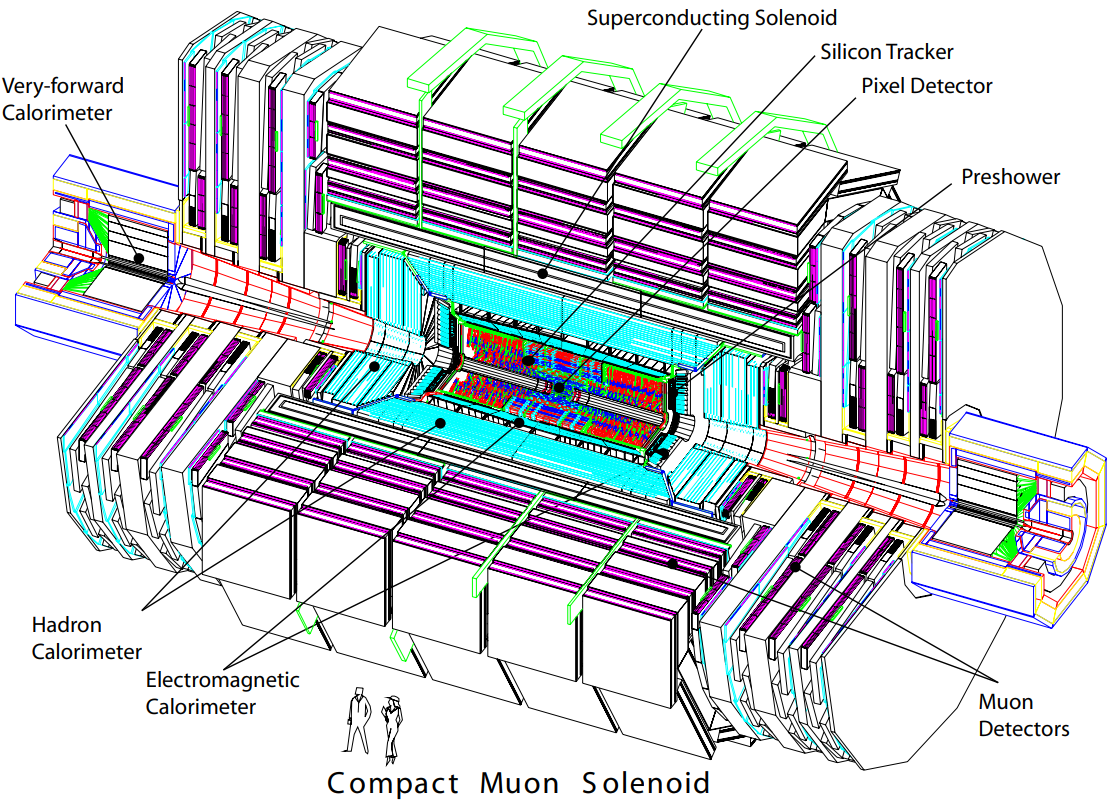
\includegraphics[scale=.3]{Chapter2/CMS_detector_simple.png}
    \caption[Panoramic view of the CMS detector]{Panoramic view of the CMS detector.}
    \label{detector_CMS}
  \end{figure}
\end{center}

To achieve high precision identification of the paths of deflected charged particles, the CMS employs a silicon tracker as its most inner detector to the beam pipe. This tracker system utilizes silicon strips and pixels that are divided into several layers in order to register the tracks of these particles. When a charged particle moves through one of the Tracker layers, it creates an interaction with the silicon material, producing a hit. By combining all the hits created by the particle, we can trace its trajectory, or track \cite{CMS_Exp_2008}. Further details about the tracker system can be found in the next section.\\

ECAL is a detector that measures the energy of electrons and photons by absorbing them completely. It is a hermetic, homogeneous calorimeter consisting of 61,200 lead tungstate (PbWO4) crystals mounted in the central barrel part and closed by 7,324 crystals in each of the two endcaps. The preshower detector is placed in front of the endcap crystals. The photodetectors used in the barrel are avalanche photodiodes (APDs), while vacuum phototriodes (VPTs) are used in the endcaps.\\ 

The HCAL surrounds the ECAL and together they complete a hermetic calorimetry system designed to measure jets and missing transverse energy. When hadrons, which are composite particles consisting of quarks and gluons, travel through the ECAL, they are stopped by the HCAL, to achieve  this, the HCAL is divided into four parts: the hadron forward (HF),  hadron endcap (HE), the hadron barrel (HB) and the hadron outer (HO) \cite{det_summary}.\\

The final particle that the CMS directly observes is the muon, these are about 200 times heavier than electrons and cannot be stopped by the calorimeters. To detect muons, special sub-detectors are built, which are integrated with the return yoke of the solenoid. The magnet's size enables us to measure the momentum of each muon both inside the superconducting coil by using the tracking devices and outside it with the help of the muon chambers \cite{det_summary}.

A transverse slice of the CMS detector, depicting specific particle interactions, is shown in Figure \ref{slice_CMS}.

\begin{center}
  \begin{figure}[ht]
    \centering
    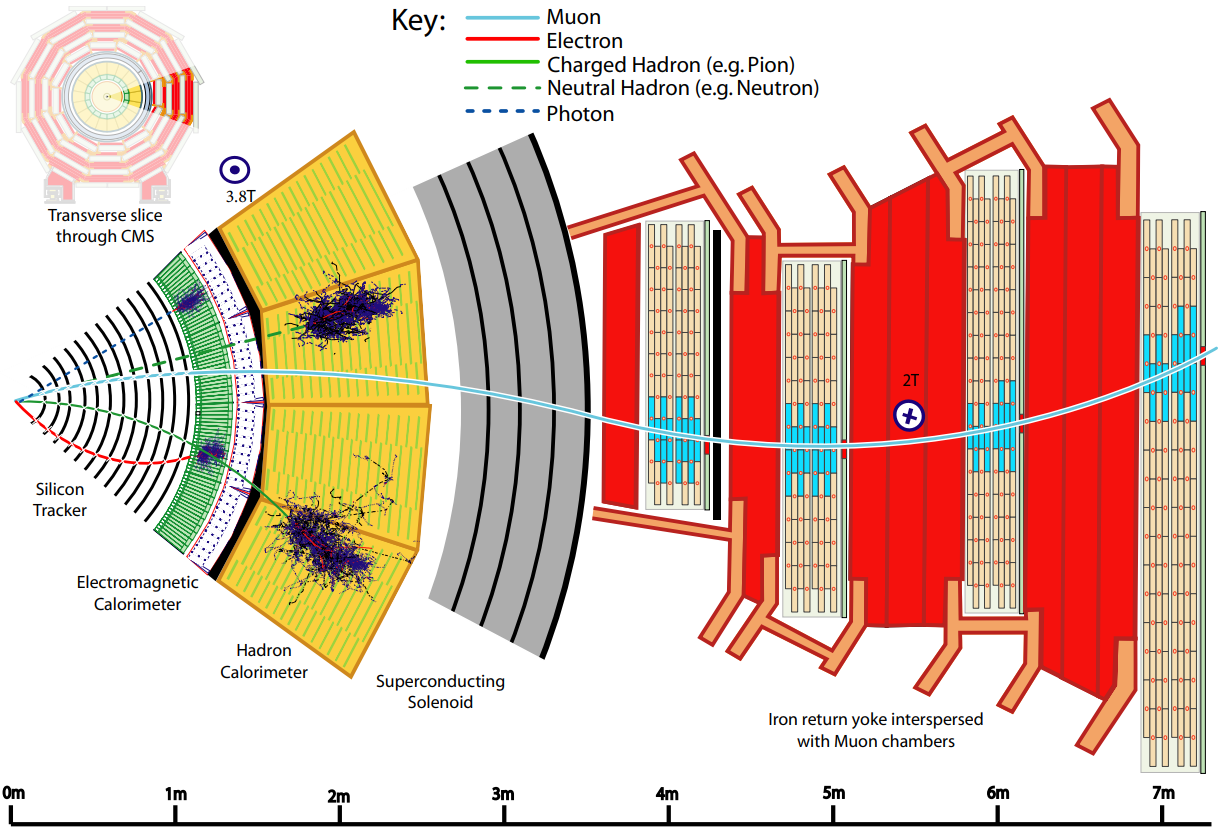
\includegraphics[scale=.3]{Chapter2/slice_det.png}
    \caption[Transverse slice view of the CMS detector]{Transverse slice of the CMS detector with some particle interactions (from the beam interaction region to the muon detector) \cite{det_summary}.}
    \label{slice_CMS}
  \end{figure}
\end{center}

The coordinate system used by the CMS is centered on the detector and has its origin at this point. The $y$-axis is oriented vertically upwards while the $x$-axis is directed radially inward, toward the center of the LHC. The z-axis aligns with the direction of the beam. Within this coordinate system, the azimuthal angle $\varphi$ is measured from the $x$-axis within the $x-y$ plane. The radial coordinate in this plane is represented by $r$. The polar angle $\theta$ is measured with respect to the z-axis. Seudorapidity $\eta$ is defined as $\eta = − ln[tan(\theta/2)]$ \cite{CMS_Exp_2008}.

\section{CMS Luminometers}
\label{Luminometers}

A total of seven systems are used for measuring luminosity at CMS. The Pixel Luminosity Telescope (PLT) and Fast Beam Conditions Monitor (BCM1F) are dedicated systems for luminosity measurement, while the hadronic forward calorimeter (HF) uses a dedicated readout on an existing system. Additionally, three other methods, the drift tube luminosity (DT), the pixel cluster counting method (PCC), and the vertex counting method (VTX), use data from existing parts of the CMS detector to perform a luminosity measurement using the main CMS DAQ system. The PCC measurement uses the data collected with the standard CMS trigger system with triggers requiring colliding bunches but not any specific event activity, known as "zero-bias" triggers. Finally, the RAMSES detectors are part of the LHC environmental protection and monitoring systems, but they can also be used to provide a luminosity measurement readout through Timber (operational data and LHC logging service) \cite{pas_18}.  A brief overview of the CMS luminometers is provided below.\\

PLT is a system designed to measure luminosity, using silicon pixel sensors. It consists of a total of 48 sensors, which are arranged into 16 "telescopes" placed at both ends of the CMS, outside the pixel endcap. Each telescope comprises three sensor planes, which are nearly parallel to the beam pipe. The PLT system measures the rate of "triple coincidences," where a hit is detected in all three planes. These coincidences typically correspond to tracks from particles originating at the interaction point. To estimate the overall mean rates for PLT, the zero-counting method is used. This method assumes that the number of observed triple coincidences follow a Poisson distribution \cite{pas_18}.\\

In Run 2, BCM1F was equipped with a total of 24 sensors mounted on the same carriages as PLT. This system included 10 silicon sensors, 10 polycrystalline diamond sensors, and 4 single-crystal diamond sensors. The BCM1F readout has a fast readout time with a 6.25 ns time resolution. The combination of precise time measurement and the location of BCM1F at 1.8 m from the center of CMS allows for the separation of hits resulting from collision products and those resulting from the machine-induced background. This is because the incoming background is separated in time from the outgoing collision products \cite{pas_18}.\\ 

HF luminosity measurement uses a dedicated readout system installed in the HF calorimeter readout electronics. Only two HF rings are used for luminosity measurement to ensure relatively uniform occupancy. Two algorithms are available: the first relies on the fraction of occupied towers (HFOC), and the second is based on the sum of the transverse energy ET (HFET)  \cite{pas_18}.\\

The DT luminosity measurement technique relies on the rate of muon track stubs in the muon barrel track finder. However, it is important to note that the DT algorithm used does not provide bunch-by-bunch measurements. Therefore, this technique can only be used for total luminosity measurements. DT measurement is generally  stable and linear so it provides a complementary offline reference measurement. The rate in DT during vdM fills is too low to allow for calibration using the vdM scan, so it is cross-calibrated to another detector \cite{pas_18}.\\

RAMSES  is a CERN radiation and environmental monitoring system. Although is not designed as a luminometer, the rate observed in this detector does function quite well as a luminosity measurement. The sensor itself is a cylindrical plastic ionization chamber filled with 3 L of air at atmospheric pressure and it primarily detects photons.  The overall rate is small, which means that it is not capable of making bunch by bunch measurements and cannot be independently calibrated using a vdM scan; however, this also means it is less affected by issues such as instability caused by radiation damage or nonlinearity \cite{pas_18}.\\

The PCC method uses the rate of pixel clusters in the CMS pixel detector to provide a luminosity measurement this method will be described in more detail in chapter 3.  

The location of the 7 luminometers in the CMS experiment are shown in Figure \ref{luminometers}.

\begin{center}
  \begin{figure}[ht]
    \centering
    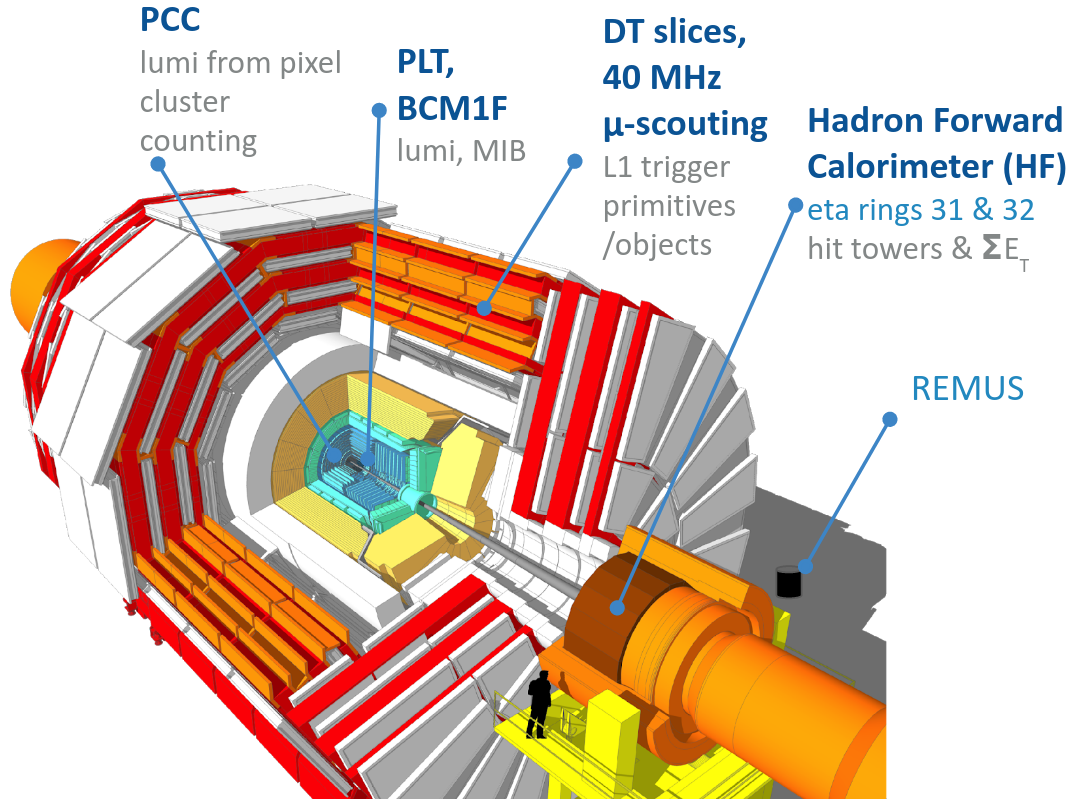
\includegraphics[scale=.3]{Chapter2/detectors.png}
    \caption[Layout of the luminometers in the CMS detector]{The seven luminometers that make up the CMS luminosity measurement system. Multiple independent systems used online: BCM1F, HFET, HFOC, PLT (independently calibrated) ,REMUS and  DT (cross-calibrated) , Pixel cluster counting is used after offline processing.}
    \label{luminometers}
  \end{figure}
\end{center}

\section{CMS Tracking System and Pixel Detector}

The tracking system plays a crucial role in precisely measuring the trajectories and momenta of charged particles generated by collisions in the LHC, as well as reconstructing secondary vertices. It has a total physical size of 5.8 m in length and 2.5 m in diameter. 
The CMS tracking detector relies on semiconductor technology, this is divided in two systems, the pixel detector and the Strip tracker \cite{CMS_Exp_2008}. In Figure \ref{strip_layout}, we can observe the pixel detector at the center, surrounded by the Strip tracker.\\

The Strip tracker is comprised of two subsystems: the first being the Tracker Inner Barrel (TIB) and Disks (TID), which are further divided into four barrel layers and three disks at each endcap. The second subsystem is the Tracker Outer Barrel (TOB), which consists of six barrel layers and the Tracker EndCaps (TEC) comprising of nine disks. The Strip tracker in total comprises of 15148 silicon modules, covering an active area of about 198$\text{m}^{2}$, and consists of 9.3 million strips \cite{CMS_Exp_2008}. \\

The innermost part of the tracking system is made up of the silicon pixel tracker, which consists of four concentric barrel layers (BPIX) and three disks on each endcap (FPIX). This component comprises a total of 124 million pixels and extends the tracker's acceptance up to a pseudorapidity of $|\eta| < 2.5$. More information about this detector is provided in the following section.

\begin{center}
  \begin{figure}[ht]
    \centering
    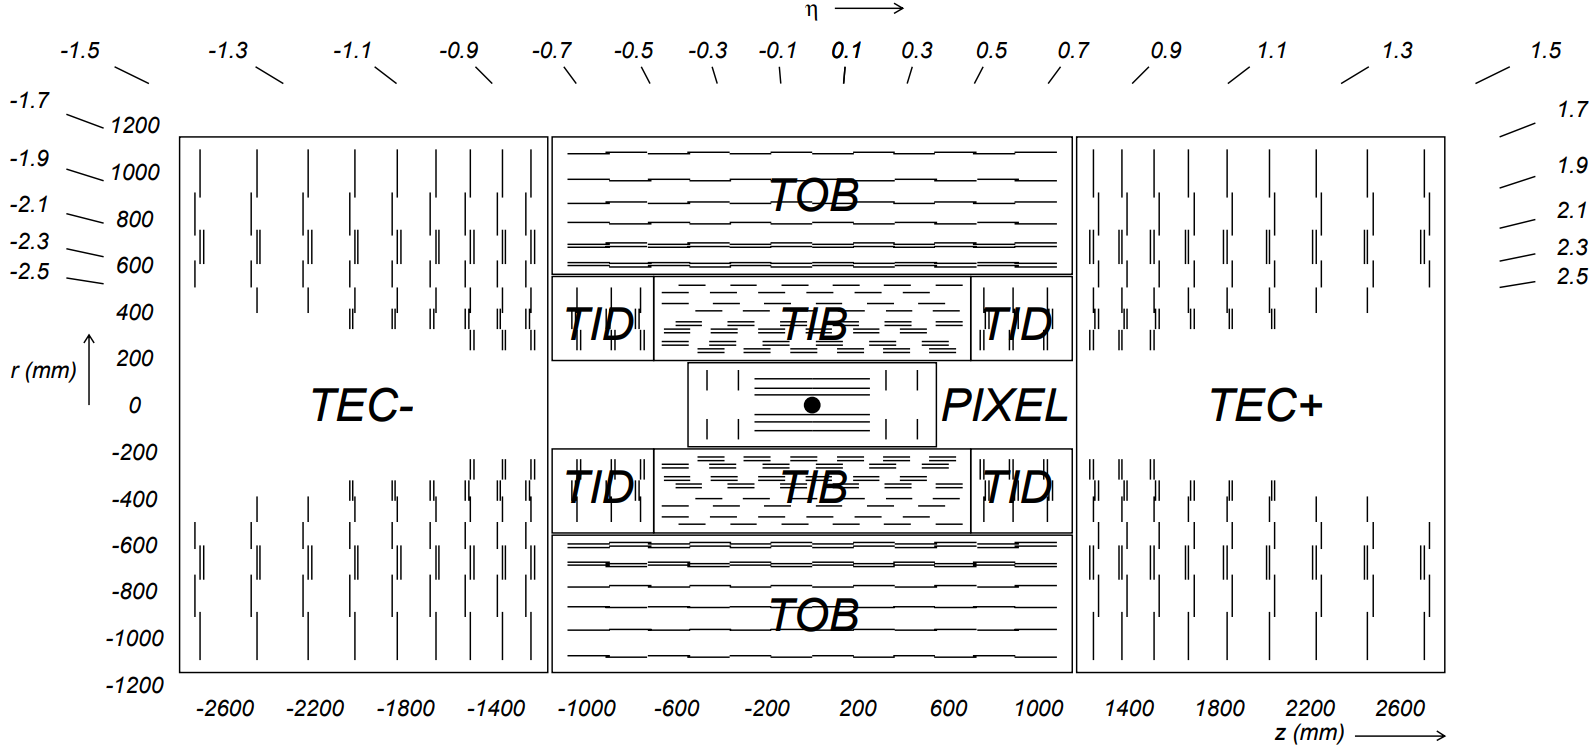
\includegraphics[scale=.23]{Chapter2/strip_layout.png}
    \caption[Schematic cross section through the CMS tracker]{Schematic cross section through the CMS tracker \cite{CMS_Exp_2008}.}
    \label{strip_layout}
  \end{figure}
\end{center}


The silicon pixel detector  forms the innermost component of the tracking system. This detector facilitates the provides complete spatial coverage over the area nearest to the interaction point, which, in turn, enables precise tracking of charged particles and vertex reconstruction. The coverage of the pixel detector is in the pseudorapidity range $(|\eta| < 2.5)$, operating in a radiation rich environment, marked by high track density \cite{phase1_Pixel_Detector}.\\

The CMS pixel detector is composed of four concentric barrel layers (L1-L4), each having radii of 29, 68, 109, and 160 mm, and three disks (D1-D3) on each end placed at distances of 291, 396, and 516 mm from the center of the detector. The entire detector is comprised of 1856 segmented silicon sensor modules.\\  

A schematic of the CMS Phase-1 pixel detector's arrangement is depicted in Figure \ref{phase1_pixel_detector} where the total silicon area spans 1.9 $\text{m}^{2}$, here The BPIX and FPIX detectors are equipped with four service half-cylinders each, with a combined length of 540 mm. These cylinders host the readout and control circuits, and provide guidance for the power lines and cooling tubes of the detector.

\begin{center}
  \begin{figure}[h]
    \centering
    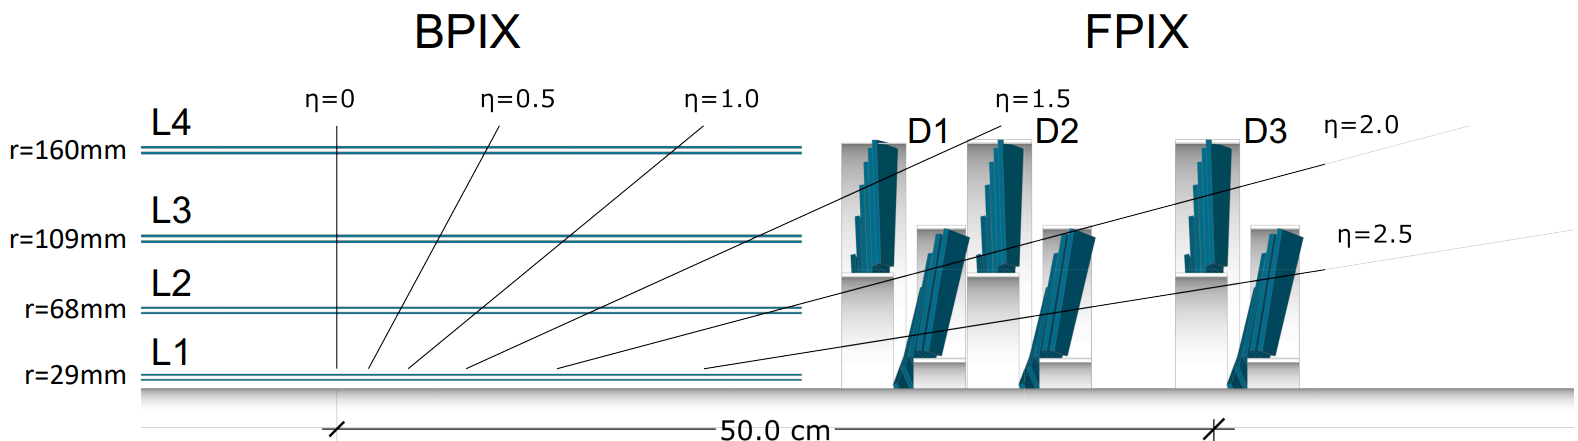
\includegraphics[scale=.26]{Chapter2/phase1_PixelDetector.png}
    \caption[CMS Phase-1 pixel detector]{Layout of the CMS Phase-1 pixel detector in longitudinal view\cite{phase1_Pixel_Detector}.}
    \label{phase1_pixel_detector}
  \end{figure}
\end{center}

The BPIX detector is divided into two independent halves that are self-sufficient mechanically. Each half comprises of a half detector and two service half-cylinders. The BPIX detector is made up of 1184 segmented silicon sensor modules where the orientation of the surface of each module is parallel to the magnetic field, in both halves.\\

In contrast to the BPIX detector, the FPIX detector is split into four quadrants, which are mechanically independent from each other. Each quadrant is composed of three half-disks that are contained within a service half-cylinder. The sensor orientation is such that the longer side of the pixel is aligned radially. The FPIX detector contains a total of 672 segmented silicon sensor modules that are subdivided into inner and outer half-rings, supporting 22 and 34 modules, respectively  \cite{phase1_Pixel_Detector}.\\

A pixel detector module is composed of a flat silicon sensor with a dimension of 18.6 $\times$ 66.6 $\text{mm}^{2}$, which contains an active area of 116.2 $\times$ 64.8 $\text{mm}^{2}$. The sensor is comprised of 160$\times$416 pixels that are bump-bonded to an array of 2 by 8 readout chips (ROC's). Each ROC contains 4160 readout channels, responsible for measuring the pulse height of each pixel. In total, the detector has 124 million readout channels. The standard pixel size is 100$\times$150 $\mu m^{2}$.

\begin{center}
  \begin{figure}[h]
    \centering
    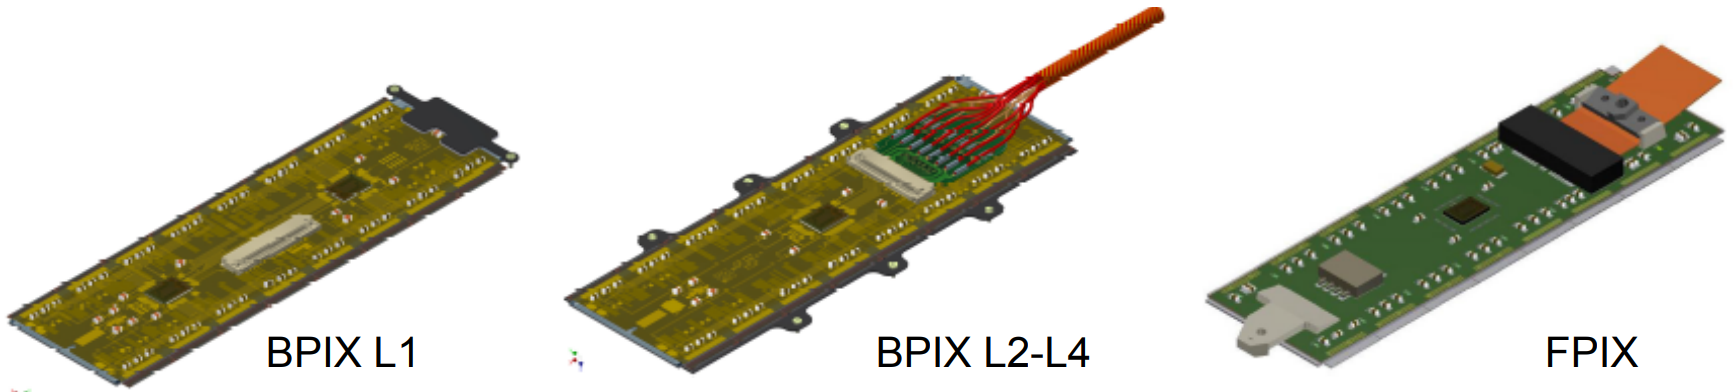
\includegraphics[scale=.2]{Chapter2/modules_drawing.png}
    \caption[Types of modules in the pixel detector]{ These are illustrations of the pixel detector modules used in the BPIX L1 (left), BPIX L2-L4 (middle), and FPIX (right) detectors \cite{phase1_Pixel_Detector}.}
    \label{modules_drawing}
  \end{figure}
\end{center}

Figure \ref{modules_drawing} illustrates the modules of the CMS Phase-1 pixel detector \cite{phase1_Pixel_Detector}, while Figure \ref{module and hit} on the left depicts the layout of the silicon sensor connected to the readout chip. On the right side of Figure \ref{module and hit}, a charged particle can be seen passing through a pixel, providing enough energy to eject electrons from the silicon atoms. A voltage applied to the sensor allows the collection of these charges as a small electric signal, which is then amplified by an electronic readout chip.

\begin{center}
  \begin{figure}[h]
    \centering
    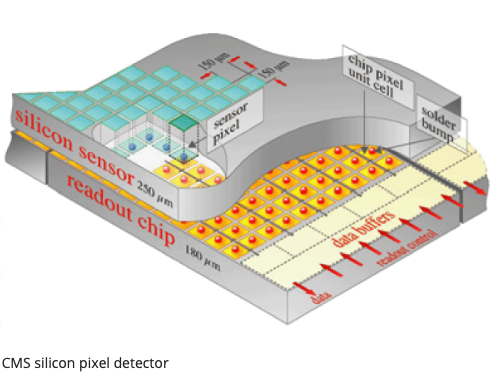
\includegraphics[scale=.3]{Chapter2/PixelSensor.png} 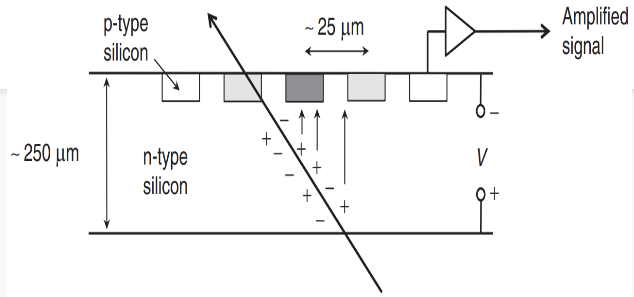
\includegraphics[scale=.3]{Chapter2/hit.png}
    \caption[Schematic view of a pixel sensor and its connection to the readout channels]{ left: layout pixel sensor connected to a readout chip , right: hits detection in a corresponding  pixel sensor \citep{thomson_2013}. }
    \label{module and hit}
  \end{figure}
\end{center}

\section{Pixel Cluster Reconstruction}

The track reconstruction process involves several steps. Firstly, the signals above a specific threshold in the pixel channels are identified and utilized to create clusters. Each cluster represents the charge deposited by a single charged particle. Subsequently, the position and uncertainties of the clusters are estimated in a coordinate system that is local and orthogonal, with respect to the sensor plane \cite{Track_Reco_2014}.\\

To be considered a valid cluster, each one should have a charge of at least 4000 electrons \cite{Track_Reco_2014,phase1_Pixel_Detector}. The minimum-ionizing particles (MIPs) passing through a silicon sensor with a 285 $\mu \text{m}$ thickness typically deposit an energy equivalent to about 21,000 electrons when they are normally incident. However, this charge is often spread over more than one pixel due to Lorentz drift,  which causes the electrons to be pushed due to the force generated by the electromagnetic field, leading to charge clusters.\\

Figure \ref{cluster}  shows an example of how a pixel cluster is constructed. Each square in the figure represents a pixel. The red pixels indicate that they have the required charge up to 2000 electrons to be considered valid pixels and are therefore included in the cluster. On the other hand, the green pixels correspond to charge depositions below the 2000 electron threshold and are not included in the cluster.
The dotted blue line in the figure represents the trajectory of the particle traveling parallel to the x-z plane. As it travels, it activates pixels in its path precisely, as well as pixels that are deviated from its trajectory due to the Lorentz drift \cite{Pixel_Hit_Reconstruction}.\\

\begin{center}
  \begin{figure}[h]
    \centering
    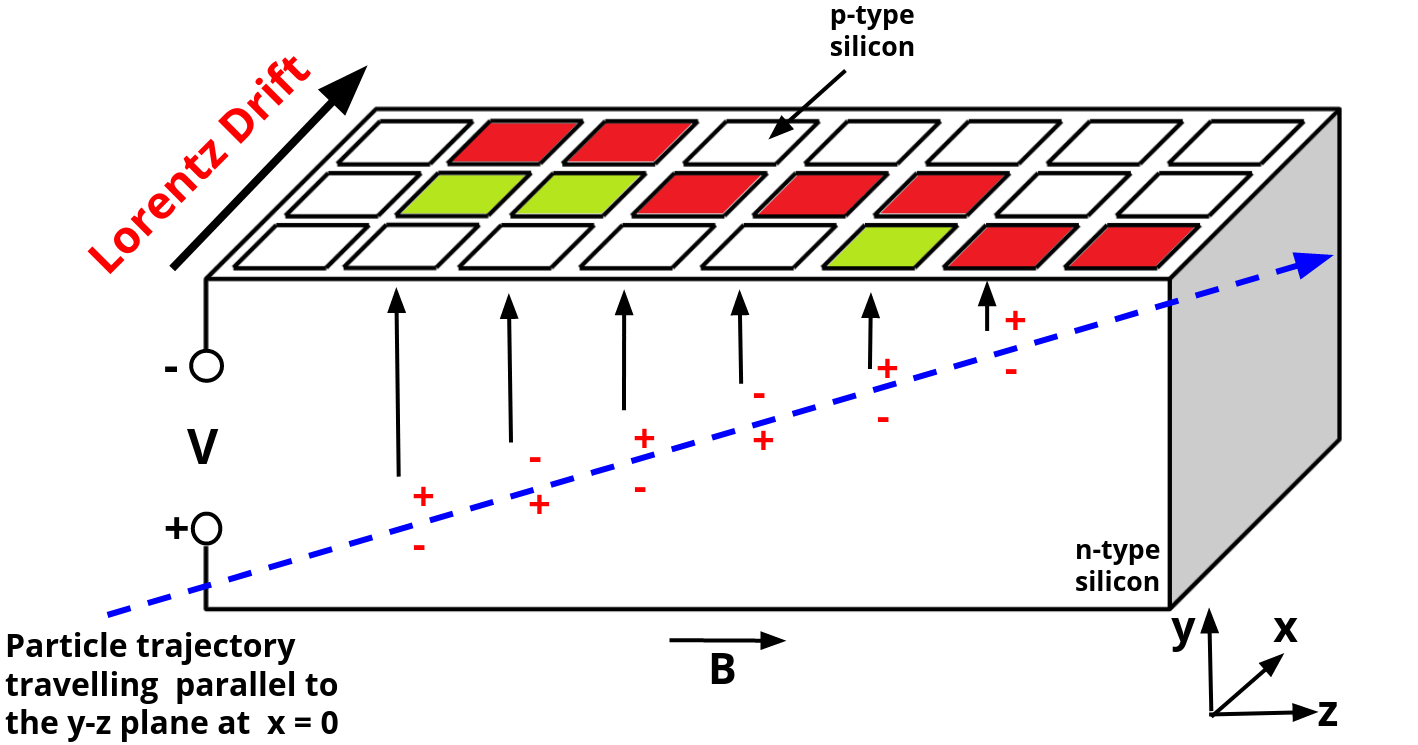
\includegraphics[scale=.25]{Chapter2/pixel_cluster.png} 
    \caption[Construction of a pixel cluster]{ The figure illustrates a pixel cluster example with a total charge up of 4,000 electrons, required to be a valid cluster. The red pixels have the required charge while the green one does not.}
    \label{cluster}
  \end{figure}
\end{center}


\section{Pixel Cluster Counting method}
\label{Pixel Cluster Counting method}

The PCC method is an offline technique that provides a luminosity measurement using the rate of pixel clusters. Due to the large area of the pixel detector and the relatively low occupancy of its sensors, the probability of a single pixel being struck by two charged particles from the same bunch crossing is extremely low. This high granularity and low occupancy result in an excellent linear response to pile-up (\(\mu\), the number of interactions per bunch crossing) \cite{PCC_PAS_12_001}. On average, the detector occupancy (# hit pixels/# total pixels) is less than 0.1\% \cite{lumi_precise_2015_2016}.  
Although the statistical precision per Lumisection (23-second period) is lower than that of online luminometers due to CMS trigger bandwidth limitations, PCC still provides a linear measurement with good precision over time. When integrated over longer periods, it delivers a stable and highly precise luminosity measurement.  

Figure \ref{pileup} shows a simulation with pp collision zero-bias events with the pixel cluster counting rate as a function of pileup in the pileup range observed in Run 2 from 0 to about 50 $\mu$. Where the mean number of pixel clusters is of the order of  111 per event. The red curve is a first-order polynomial fit with slope, the results indicate a high level of agreement, as evidenced by the estimated goodness-of-fit $\chi^{2}$ per degree of freedom (dof) of approximately 0.5, showing that the PCC rate is highly linear in this range under simulated conditions \cite{ Phase2_Upgrade,lumi_precise_2015_2016}.


\begin{center}
  \begin{figure}[h!]
    \centering
    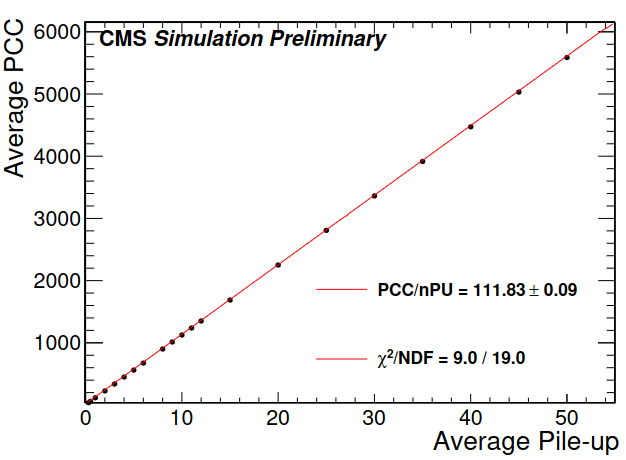
\includegraphics[scale=.35]{Chapter3/pileup_lineality.png} 
    \caption[PCC linearity with pile-up]{ Linearity of pixel cluster counting over the pileup range observed in Run 2 (from 0 to about 50) from simulation. The red line is a linear fit to the points \cite{Phase2_Upgrade} }
    \label{pileup}
  \end{figure}
\end{center}

For physics conditions, two data streams are recorded via the CMS DAQ: "zero-bias" and "random." The zero-bias stream consists of triggered data for colliding bunches at a bandwidth of approximately 1.5 kHz, while the random stream collects triggered data from all bunch crossings at a bandwidth of 500 Hz. The luminosity measurement is performed using the zero-bias data, whereas the random trigger helps evaluate background contributions.  

Under vdM conditions, a special trigger mode is employed to achieve higher data rates for PCC. This mode focuses on a selected set of five colliding bunch crossings, as detailed for each year in the next chapter, ensuring the necessary statistical precision.  

To derive the luminosity measurement from the PCC method, the mean number of pixel clusters per event is computed by averaging over several zero-bias events. This value is given by:

\begin{equation}
\left < N_{\text{cluster}} \right > \equiv \left < N_{\text{cluster}/\text{interaction}} \right > \mu
\end{equation}

Where the pile-up ($\mu$) is determined by the minimum-bias cross section: 

\begin{equation}
\mu = \frac{\sigma_{\text{minBias}}}{f} \cdot \mathcal{L}_{inst}
\end{equation}

where $f$ is the LHC revolution frequency and $\mathcal{L}_{inst}$ is the single bunch instantaneous luminosity (SBIL). The minimum bias cross section $\sigma_{\text{minBias}}$ here is related to the PCC visible cross section by the mean number of clusters per interaction:

\begin{equation}
\sigma_{vis}= \left < N_{\text{cluster}/\text{interaction}} \right >\cdot \sigma_{\text{minBias}}
\end{equation}

Combining everything, the PCC luminosity measurement is obtained as:

\begin{equation}
\mathcal{L}_{inst}=\frac{\left < N_{\text{cluster}} \right> f}{\sigma_{vis}}
\end{equation}

In the PCC measurement, the innermost layer (Layer 0) of the pixel detector is excluded due to significant dynamic inefficiency effects, as at high instantaneous luminosities, the hit efficiency decreases because the readout chip cannot process all hits in time. For PCC rate measurements, only the pixel detector modules that remain stable throughout the entire data-taking period (year) are used. Modules known to be defective or significantly affected by the limited size of the readout buffer are excluded from the analysis. The final number of excluded modules, referred to as "veto modules," is detailed for each year in the next chapter.

%This method is capable of providing a precise luminosity measurement over longer time periods, but it cannot do so for a single luminosity section (23 seconds) as is possible with online luminometers. The reason for this limitation is the limited CMS trigger bandwidth available for collecting data \cite{pas_18}. A detailed discussion on this topic can be found in the next chapter.\\

%PCC si calcula lumi por cada lumi section.  Esto no tiene que ver con online vs offline.  PCC es un offline luminometro, quiere decir que los datos llegan tarde.  Con PCC solo podemos calcular lumi cada lumi section, debido a la baja estadistica (por la lectura de los datos de zero bias).  otros luminometros tienen precision con NB4 (HF, PLT, BCM1F).  

